\documentclass[11pt, a4paper]{article}

\usepackage[margin=2cm]{geometry}
\usepackage{amsmath, amssymb}
\usepackage{graphicx}
\usepackage{booktabs}
\usepackage{array}
\usepackage{xcolor}
\usepackage{hyperref}
\usepackage{caption}
\usepackage{subcaption}
\usepackage{parskip}
\usepackage{titlesec}
\usepackage{enumitem}
\usepackage{fancyhdr}

\pagestyle{fancy}
\fancyhf{}
\rhead{\small Problem 1.2 --- VAE Loss Function}
\lhead{\small MNIST Experiments}
\rfoot{\small\thepage}

\definecolor{myblue}{RGB}{31,119,180}
\hypersetup{colorlinks=true, linkcolor=myblue, urlcolor=myblue}

\titleformat{\section}{\normalsize\bfseries}{}{0em}{}[\titlerule]
\titleformat{\subsection}{\small\bfseries}{}{0em}{}
\titlespacing{\section}{0pt}{6pt}{3pt}
\titlespacing{\subsection}{0pt}{4pt}{2pt}

\setlength{\parskip}{3pt}
\captionsetup{font=small, skip=3pt}
\setlist{noitemsep, topsep=2pt, leftmargin=1.5em}

% ─────────────────────────────────────────────────────────────────────────────
\begin{document}

\begin{center}
  {\large\textbf{Problem 1.2 --- The VAE Loss Function}}
\end{center}
\vspace{-0.3em}\hrule\vspace{0.6em}

% ─────────────────────────────────────────────────────────────────────────────
\section{Background and Objective}

A \textbf{Variational Autoencoder} (VAE) maps each input to a \emph{distribution}
in latent space ($\mu$, $\log\sigma^2$) rather than a point, then decodes a sample
drawn from that distribution. Training minimises two objectives: (1)
\textbf{Reconstruction Loss} --- how faithfully the decoder reproduces the input,
and (2) \textbf{KL Divergence} --- a regulariser pulling the latent distribution
toward $\mathcal{N}(0,I)$. The goal here is to implement this combined loss, train
on MNIST for 20 epochs, plot all three loss components, and analyse the effect of
$\beta$ on reconstruction sharpness.

% ─────────────────────────────────────────────────────────────────────────────
\section{Loss Function Formulation}

\[
  \mathcal{L}_{\text{total}} = \mathcal{L}_{\text{recon}} + \beta\cdot\mathcal{L}_{\text{KLD}}
\]

\subsection*{Reconstruction Loss --- Binary Cross-Entropy (BCE)}
\[
  \mathcal{L}_{\text{recon}}
    = -\frac{1}{N}\sum_{i=1}^{N}\sum_{d=1}^{D}
      \bigl[x_{id}\log\hat{x}_{id} + (1-x_{id})\log(1-\hat{x}_{id})\bigr]
\]
$x_{id}$: true pixel, $\hat{x}_{id}$: decoder output, $N$: batch size, $D=784$.

\subsection*{KL Divergence}
\[
  \mathcal{L}_{\text{KLD}}
    = -\frac{1}{2N}\sum_{i=1}^{N}\sum_{j=1}^{d}
      \bigl(1 + \log\sigma_{ij}^2 - \mu_{ij}^2 - \sigma_{ij}^2\bigr)
\]

\subsection*{Role of $\beta$}
$\beta=1$: original VAE \cite{kingma2013auto}. $\beta>1$ ($\beta$-VAE): more
disentangled latent space, lower reconstruction quality. $\beta<1$: sharper
reconstructions, less structured latent space.

% ─────────────────────────────────────────────────────────────────────────────
\section{Model Architecture}

Fully connected (no convolutions). Latent dim: 20. Optimiser: Adam ($10^{-3}$). Batch: 128.

\begin{center}\small
\begin{tabular}{lll}
  \toprule
  \textbf{Component} & \textbf{Layer} & \textbf{Dimensions} \\
  \midrule
  Encoder & FC + ReLU & $784\to400$ \\
          & FC (mean / log-var) & $400\to20$ each \\
  Reparam. & $z=\mu+\varepsilon\cdot\sigma,\;\varepsilon\sim\mathcal{N}(0,I)$ & dim 20 \\
  Decoder & FC + ReLU, FC + Sigmoid & $20\to400\to784$ \\
  \bottomrule
\end{tabular}
\end{center}

% ─────────────────────────────────────────────────────────────────────────────
\section{Results --- Baseline ($\beta=1.0$)}

\begin{figure}[h]
  \centering
  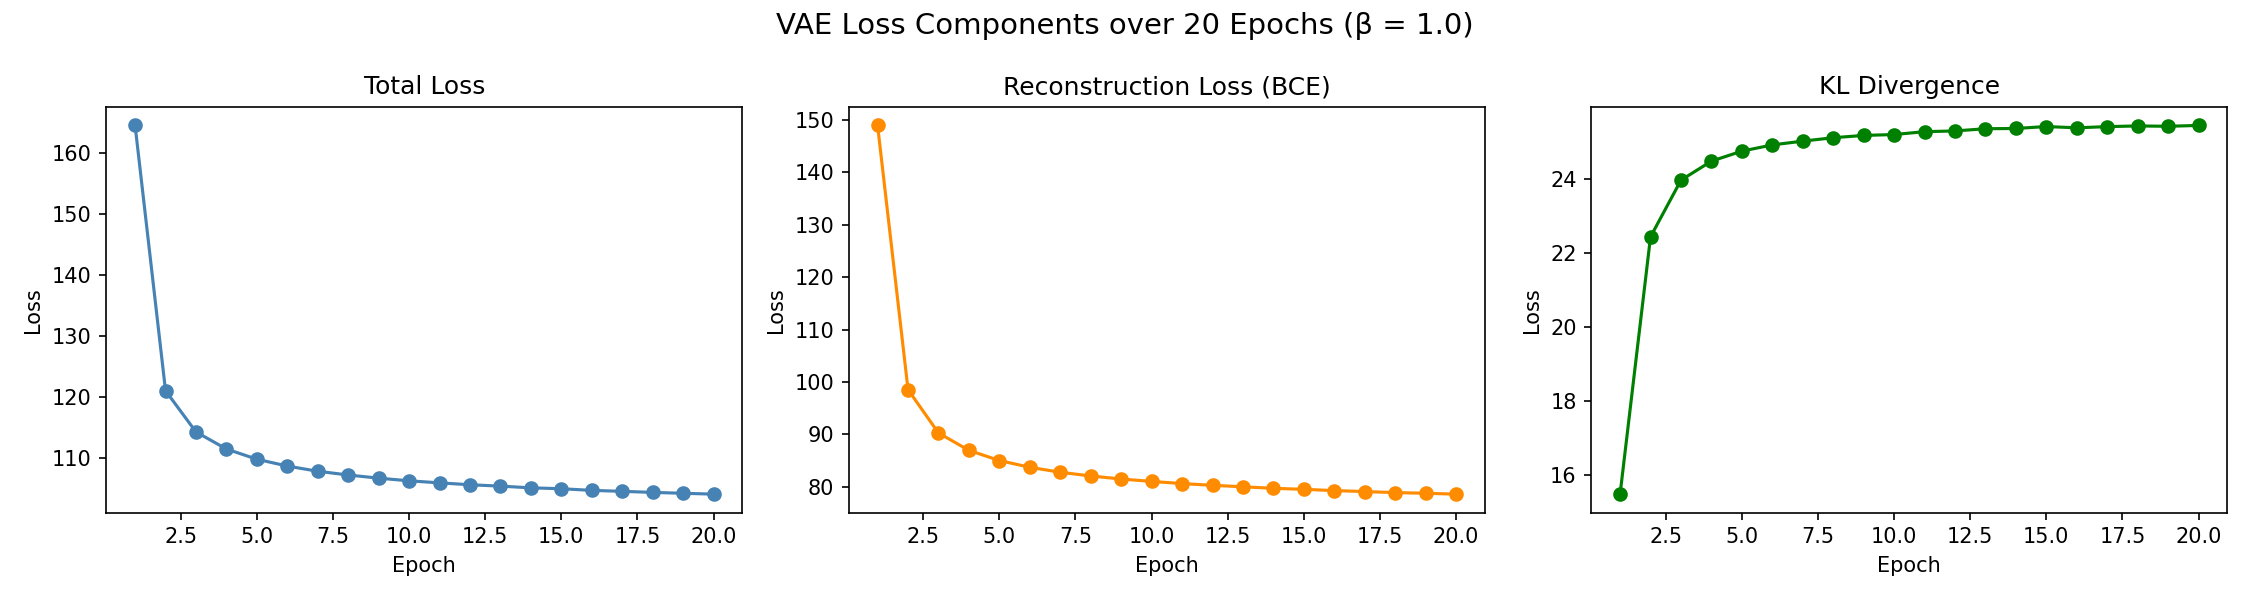
\includegraphics[width=\linewidth]{loss_plot_beta1.png}
  \caption{Total, Reconstruction (BCE), and KL Divergence over 20 epochs ($\beta=1.0$).}
\end{figure}

\begin{center}\small
\begin{tabular}{ccccp{5cm}}
  \toprule
  \textbf{Epoch} & \textbf{Total} & \textbf{Recon} & \textbf{KLD} & \textbf{Notes}\\
  \midrule
  1  & 164.45 & 148.98 & 15.47 & Fast initial drop \\
  5  & 109.73 &  84.99 & 24.74 & KLD plateauing \\
  10 & 106.19 &  81.00 & 25.19 & Slow convergence \\
  20 & 104.01 &  78.58 & 25.43 & Final values \\
  \bottomrule
\end{tabular}
\end{center}

\textbf{Key observations:}
\begin{itemize}
  \item Total and Recon losses drop sharply in epochs 1--2, then converge slowly.
  \item KLD \emph{rises} from $\approx15$ to a plateau near $25$ --- the encoder
        gradually uses more latent capacity as reconstruction pressure increases.
\end{itemize}

% ─────────────────────────────────────────────────────────────────────────────
\section{Effect of $\beta$ on Reconstruction Sharpness}

\begin{figure}[h]
  \centering
  \begin{subfigure}{\linewidth}
    \centering
    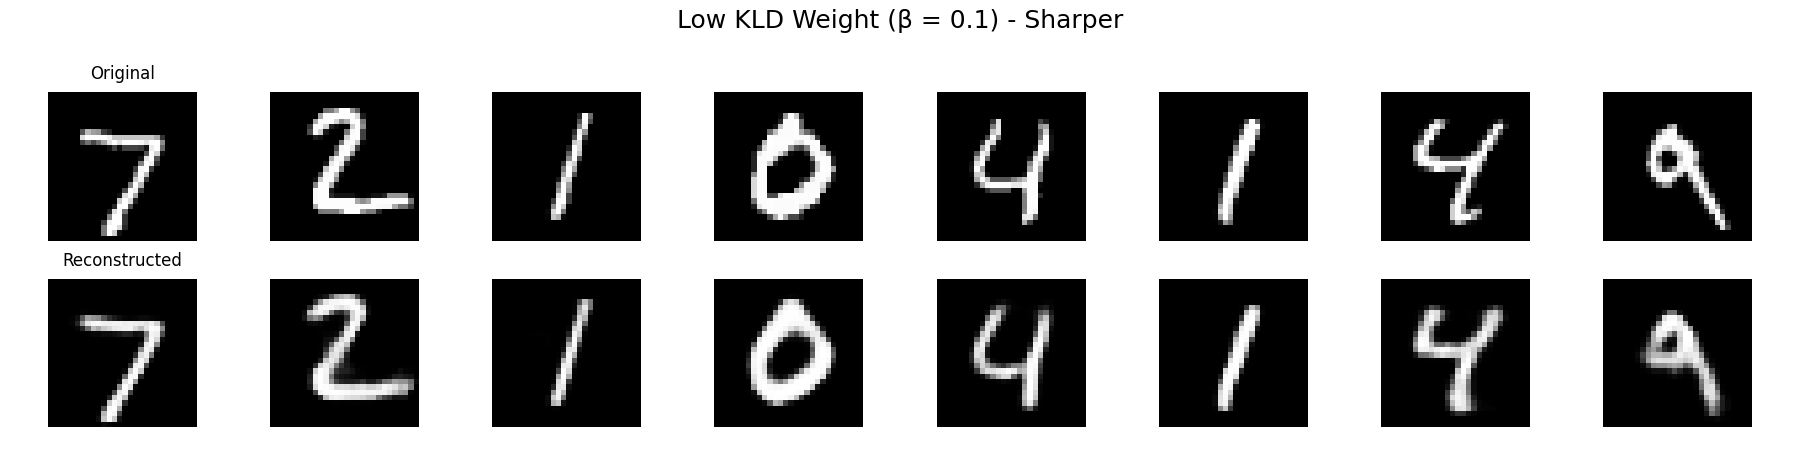
\includegraphics[width=\linewidth]{Low_KLD_Weight_(β_=_0.1)_-_Sharper.png}
    \caption{$\beta=0.1$ --- low KLD weight. Top: originals. Bottom: reconstructions.}
  \end{subfigure}\vspace{0.5em}
  \begin{subfigure}{\linewidth}
    \centering
    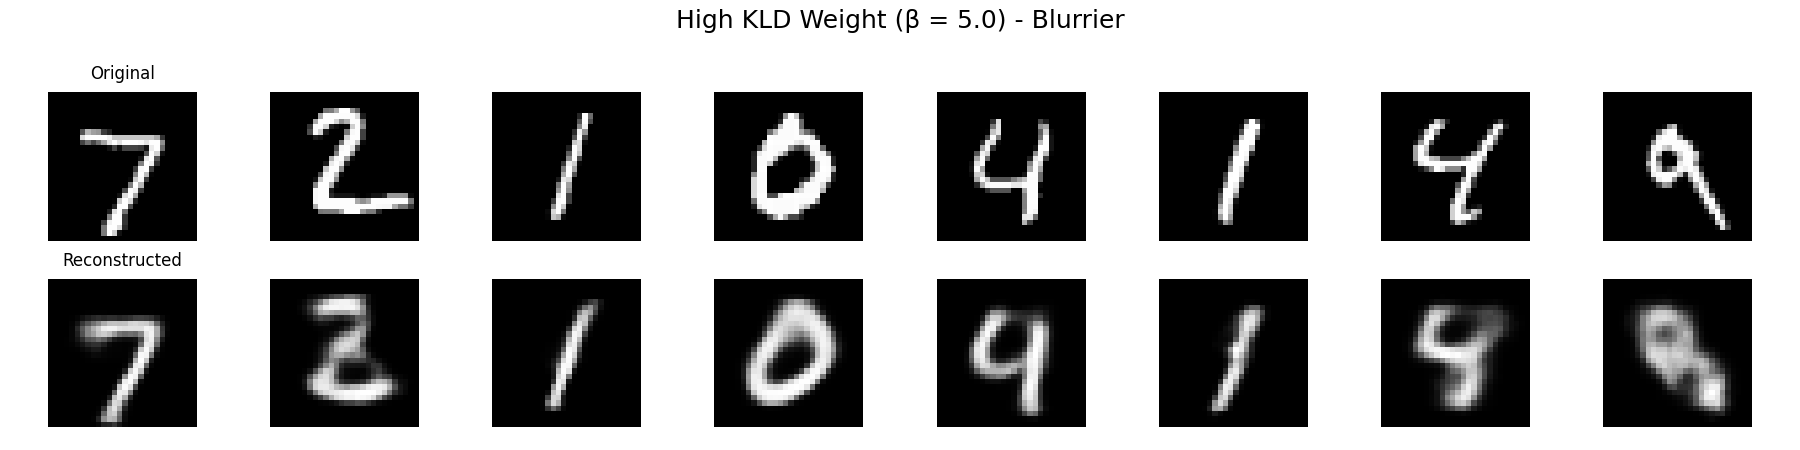
\includegraphics[width=\linewidth]{High_KLD_Weight_(β_=_5.0)_-_Blurrier.png}
    \caption{$\beta=5.0$ --- high KLD weight. Top: originals. Bottom: reconstructions.}
  \end{subfigure}
  \caption{Reconstruction quality: low vs.\ high $\beta$.}
\end{figure}

\begin{figure}[h]
  \centering
  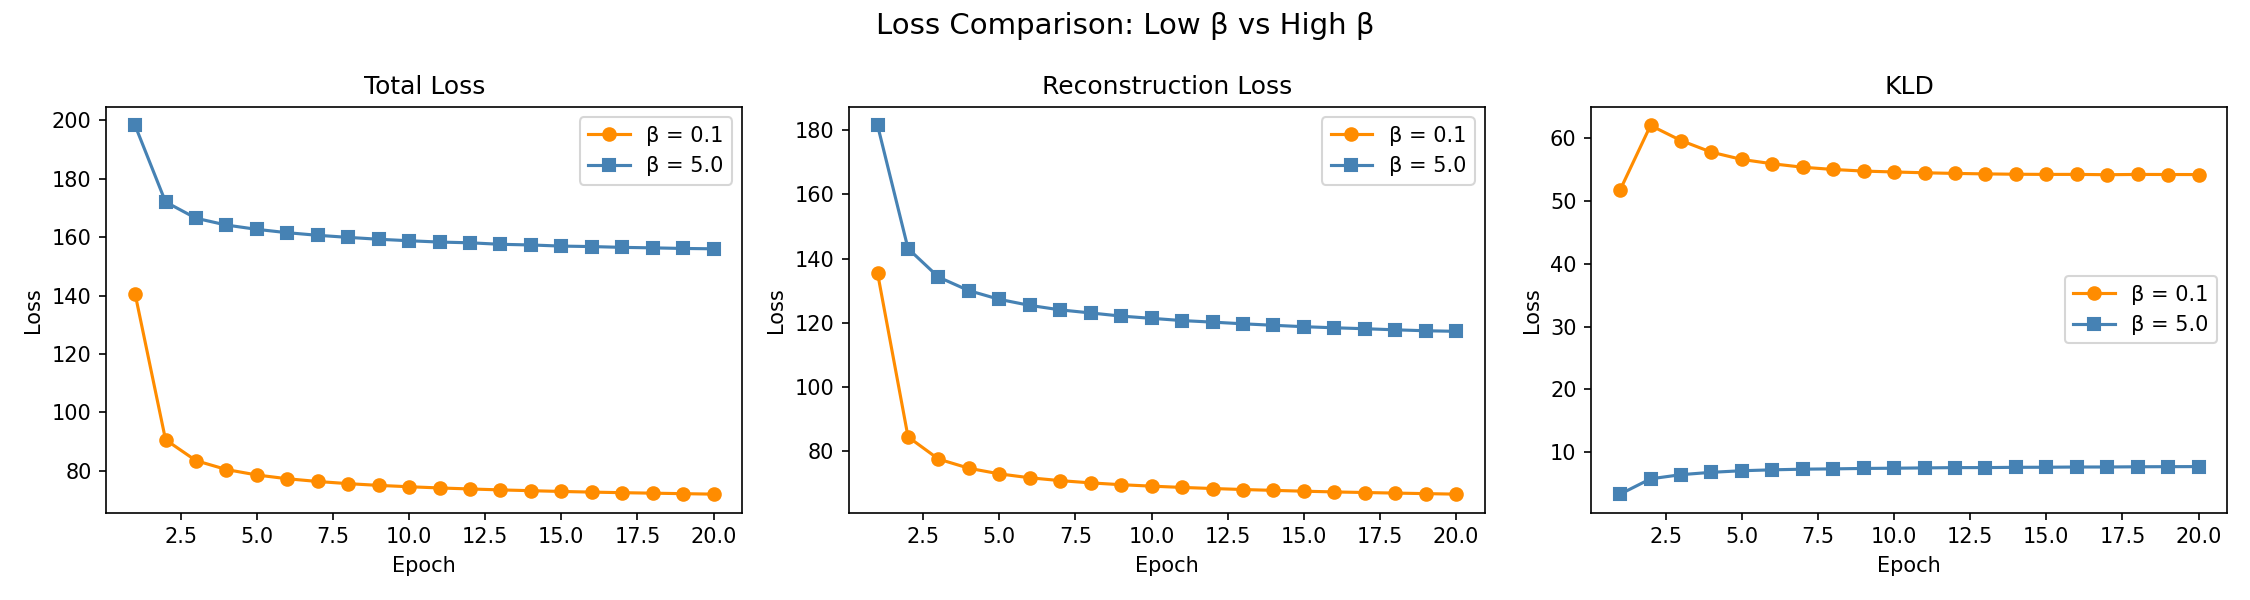
\includegraphics[width=\linewidth]{loss_comparison.png}
  \caption{Loss curves: $\beta=0.1$ (orange) vs.\ $\beta=5.0$ (blue) over 20 epochs.}
\end{figure}

\subsection*{Numerical summary at epoch 20}
\begin{center}\small
\begin{tabular}{lccc}
  \toprule
  \textbf{Model} & \textbf{Total} & \textbf{Recon} & \textbf{KLD}\\
  \midrule
  $\beta=0.1$ & 72.05 & 66.63 & 54.20 \\
  $\beta=1.0$ (baseline) & 104.01 & 78.58 & 25.43 \\
  $\beta=5.0$ & 156.03 & 117.37 &  7.73 \\
  \bottomrule
\end{tabular}
\end{center}

% ─────────────────────────────────────────────────────────────────────────────
\section{Observation and Analysis}

\subsection*{What happens to sharpness when $\beta$ is increased?}
\begin{center}\small
\begin{tabular}{>{\bfseries}p{1.8cm} p{2.5cm} p{2.5cm} p{6.5cm}}
  \toprule
  $\beta$ & Recon Loss & KLD & Image quality \\
  \midrule
  Low (0.1)  & Lower ($\approx67$)  & Higher ($\approx54$) & Sharper, crisper digits \\
  High (5.0) & Higher ($\approx117$) & Lower ($\approx8$)   & Blurry, detail lost \\
  \bottomrule
\end{tabular}
\end{center}

\textbf{Low $\beta$:} Reconstruction dominates. The encoder places latent codes
freely in $\mathbb{R}^{20}$, giving the decoder rich, precise information ---
producing sharp outputs. High KLD ($\approx54$) confirms the posterior deviates
from $\mathcal{N}(0,I)$.

\textbf{High $\beta$:} KLD dominates, forcing all inputs toward $\mathcal{N}(0,I)$.
The compressed latent code carries little input-specific detail, so the decoder
produces blurry, averaged reconstructions. Low KLD ($\approx8$) confirms tight
regularisation.

\subsection*{The Fundamental VAE Trade-off}
\[
  \underbrace{\text{Reconstruction fidelity}}_{\text{lower }\beta}
  \;\longleftrightarrow\;
  \underbrace{\text{Latent-space regularity}}_{\text{higher }\beta}
\]
A well-regularised latent space benefits \emph{generation} and disentanglement
but hurts \emph{reconstruction sharpness}. The choice of $\beta$ depends on the
downstream task.

% ─────────────────────────────────────────────────────────────────────────────
\section{Summary}
\begin{enumerate}
  \item VAE loss = BCE reconstruction + $\beta\cdot$KLD regularisation.
  \item At $\beta=1$: total loss $164\to104$; KLD rises $15\to25$; Recon $149\to79$.
  \item Higher $\beta$ $\Rightarrow$ lower KLD, higher recon error, \emph{blurrier} images.
  \item Lower $\beta$ $\Rightarrow$ higher KLD, lower recon error, \emph{sharper} images.
\end{enumerate}

\begin{thebibliography}{9}
\bibitem{kingma2013auto}
  D.~P.~Kingma and M.~Welling, ``Auto-Encoding Variational Bayes,'' \textit{ICLR}, 2014.
\bibitem{higgins2017beta}
  I.~Higgins et~al., ``$\beta$-VAE: Learning Basic Visual Concepts\ldots,'' \textit{ICLR}, 2017.
\end{thebibliography}

\end{document}